\documentclass[12pt,a4paper]{article}
\usepackage[utf8]{vietnam}
\usepackage{amsmath,amssymb}
\usepackage{geometry}
\geometry{top=1.5cm,bottom=1.2cm,left=1.4cm,right=1.4cm,headheight=28pt,headsep=12pt,footskip=18pt}
\usepackage{tikz}
\usepackage{xcolor}
\usepackage{enumerate}
\usepackage{graphicx}
\usepackage[version=4]{mhchem}
\usepackage{fancyhdr}
\usepackage{ex_test}

\renewcommand{\baselinestretch}{0.96}
\setlength{\parskip}{0pt}

\definecolor{hfRed}{RGB}{211,47,47}
\definecolor{hfGreen}{RGB}{139,195,144}

\pagestyle{fancy}
\fancyhf{}
\fancyhead[L]{\small\itshape\color{hfRed} Tài liệu lưu hành nội bộ}
\fancyhead[R]{\small\itshape\color{hfRed} Thầy \textbf{TRẦN VĂN THẠNH} - 0777.470.803}
\renewcommand{\headrulewidth}{0.8pt}
\renewcommand{\headrule}{\hbox to\headwidth{\color{hfGreen}\leaders\hrule height \headrulewidth\hfill}}

\fancyfoot[L]{\small\itshape\color{hfRed} CS1: 6/15 Nguyễn Hoàng, P. Kim Long, TP Huế \quad|\quad CS2: 24 Đặng Thái Thân, TP Huế}
\fancyfoot[R]{\small\bfseries\color{hfRed} Trang \thepage}
\renewcommand{\footrulewidth}{0.8pt}
\renewcommand{\footrule}{\hbox to\headwidth{\color{hfGreen}\leaders\hrule height \footrulewidth\hfill}}

\fancypagestyle{firstpage}{
  \fancyhf{}
  \renewcommand{\headrulewidth}{0pt}
  \fancyfoot[L]{\small\itshape\color{hfRed} CS1: 6/15 Nguyễn Hoàng, P. Kim Long, TP Huế \quad|\quad CS2: 24 Đặng Thái Thân, TP Huế}
  \fancyfoot[R]{\small\bfseries\color{hfRed} Trang \thepage}
  \renewcommand{\footrulewidth}{0.8pt}
  \renewcommand{\footrule}{\hbox to\headwidth{\color{hfGreen}\leaders\hrule height \footrulewidth\hfill}}
}

\begin{document}
\thispagestyle{firstpage}

\noindent
\begin{minipage}[t]{0.44\textwidth}
	\centering\fontsize{10pt}{12pt}\selectfont
	\textbf{SỞ GIÁO DỤC VÀ ĐÀO TẠO THỪA THIÊN HUẾ}\\
	\textbf{ĐỀ CHÍNH THỨC}\\
	\textit{(Đề thi có 04 trang)}
\end{minipage}\hfill
\begin{minipage}[t]{0.54\textwidth}
	\centering\fontsize{10.5pt}{13pt}\selectfont
	\textbf{ĐỀ KIỂM TRA ĐỊNH KỲ CHƯƠNG 3 (ĐẠI CƯƠNG HÓA HỌC HỮU CƠ)}\\
	\textbf{MÔN: HOÁ HỌC - LỚP 11}\\
	\textit{Thời gian làm bài: 45 phút, không kể thời gian phát đề}
	
	\smallskip
	\fbox{\textbf{MÃ ĐỀ: 109}}
\end{minipage}

\smallskip
\begin{center}
	{\color{hfRed}\textbf{\large (BẢN GIÁO VIÊN -- CÓ LỜI GIẢI CHI TIẾT)}}
\end{center}

\smallskip
\noindent\hrulefill
\smallskip

\noindent\textbf{Họ, tên thí sinh:} \dotfill\ \textbf{Lớp:} \dotfill\ \textbf{Số báo danh:} \dotfill

\smallskip
\noindent\textit{(Cho biết nguyên tử khối: H = 1; C = 12; N = 14; O = 16; F = 19; Na = 23; Mg = 24; Al = 27; P = 31; S = 32; Cl = 35,5; K = 39; Ca = 40; Fe = 56; Cu = 64; Br = 80; Ag = 108).}
\smallskip

\noindent\textbf{\large PHẦN I. Câu trắc nghiệm nhiều phương án lựa chọn.}
\textit{Thí sinh trả lời từ câu 1 đến câu 18. Mỗi câu hỏi thí sinh chỉ chọn một phương án.}
\vspace{0.2cm}

\Opensolutionfile{ans}[ans-hoa11-de09gv]

\begin{ex}
Cho các chất sau: $\ce{NaHCO3}$, $\ce{CH4}$, $\ce{C2H6O}$, $\ce{CH3COONa}$, $\ce{CaC2}$, $\ce{Al4C3}$. Hợp chất nào thuộc loại hợp chất hữu cơ?
\choice
{\True $\ce{CH4}$, $\ce{C2H6O}$, $\ce{CH3COONa}$}
{$\ce{NaHCO3}$, $\ce{CaC2}$, $\ce{Al4C3}$}
{$\ce{NaHCO3}$, $\ce{CH4}$, $\ce{C2H6O}$}
{$\ce{CH4}$, $\ce{C2H6O}$, $\ce{Al4C3}$}

\loigiai{
Hợp chất hữu cơ là hợp chất của carbon (trừ $\ce{CO}$, $\ce{CO2}$, muối carbonate, cyanide, carbide,...). Do đó $\ce{CH4}$, $\ce{C2H6O}$, $\ce{CH3COONa}$ là hợp chất hữu cơ; $\ce{NaHCO3}$, $\ce{CaC2}$, $\ce{Al4C3}$ là các hợp chất vô cơ.
}
\end{ex}

\begin{ex}
Trong thành phần phân tử hợp chất hữu cơ nhất thiết phải có nguyên tố nào sau đây?
\choice
{\True carbon}
{hydrogen}
{oxygen}
{nitrogen}

\loigiai{
Theo định nghĩa, hợp chất hữu cơ là hợp chất của carbon (trừ một số hợp chất vô cơ chứa carbon), do đó trong phân tử nhất thiết phải có nguyên tố carbon.
}
\end{ex}

\begin{ex}
Phát biểu nào sau đây \textbf{không đúng} khi nói về phương pháp chưng cất?
\choice
{Phương pháp chưng cất dùng để tách các chất lỏng có nhiệt độ sôi khác nhau nhiều}
{\True Chất nào có nhiệt độ sôi thấp sẽ chuyển thành hơi muộn hơn và ít hơn}
{Chất có nhiệt độ sôi thấp hơn sẽ chuyển thành hơi sớm hơn và nhiều hơn}
{Hơi bay ra được dẫn qua ống sinh hàn làm lạnh để ngưng tụ thành chất lỏng}

\loigiai{
Chất có nhiệt độ sôi thấp hơn sẽ chuyển thành hơi sớm hơn và nhiều hơn chất có nhiệt độ sôi cao, do đó phát biểu B sai.
}
\end{ex}

\begin{ex}
Chiết là phương pháp tách chất dựa vào sự hòa tan khác nhau của ... trong hai môi trường không tan vào nhau. Cụm từ thích hợp điền vào chỗ trống là
\choice
{\True chất cần tách}
{chất lỏng}
{dung môi}
{chất tan}

\loigiai{
Phương pháp chiết dựa trên sự hòa tan khác nhau của chất cần tách trong hai pha không trộn lẫn (thường là hai chất lỏng không tan vào nhau).
}
\end{ex}

\begin{ex}
Hợp chất hữu cơ X có công thức phân tử $\ce{C_xH_yO_z}$, phân tử khối là $M$. Công thức tính giá trị của $z$ là
\choice
{$z = \dfrac{\%m_{\ce{O}}}{16} \times 100$}
{$z = \dfrac{\%m_{\ce{O}}}{M} \times 100$}
{$z = \dfrac{\%m_{\ce{O}}}{M} \times \dfrac{16}{100}$}
{\True $z = \dfrac{\%m_{\ce{O}}}{16} \times \dfrac{M}{100}$}

\loigiai{
Ta có $\%m_{\ce{O}} = \dfrac{16z}{M} \times 100\% \Rightarrow z = \dfrac{\%m_{\ce{O}} \times M}{16 \times 100} = \dfrac{\%m_{\ce{O}}}{16} \times \dfrac{M}{100}$.
}
\end{ex}

\begin{ex}
\textbf{[SBT - KNTT]} Trong phương pháp phổ khối lượng, đối với các hợp chất đơn giản, thường mảnh có giá trị $m/z$ lớn nhất ứng với mảnh ion phân tử $[\ce{M+}]$ và giá trị này bằng giá trị ....... của chất nghiên cứu. Cụm từ thích hợp điền vào chỗ trống là
\choice
{\True phân tử khối}
{nguyên tử khối}
{điện tích ion}
{khối lượng}

\loigiai{
Mảnh ion phân tử $[\ce{M+}]$ có điện tích $z = +1$ nên giá trị $m/z$ của nó bằng đúng phân tử khối của chất nghiên cứu.
}
\end{ex}

\begin{ex}
\textbf{[KNTT - SGK]} Cặp chất nào sau đây là đồng phân của nhau?
\choice
{$\ce{C2H5OH}$ và $\ce{CH3-O-C2H5}$}
{$\ce{CH3-O-CH3}$ và $\ce{CH3CHO}$}
{\True $\ce{CH3-CH2-CH2-OH}$ và $\ce{CH3-CH(OH)-CH3}$}
{$\ce{CH3-CH2-CH2-CH3}$ và $\ce{CH3-CH2-CH=CH2}$}

\loigiai{
$\ce{CH3-CH2-CH2-OH}$ (propan-1-ol) và $\ce{CH3-CH(OH)-CH3}$ (propan-2-ol) có cùng công thức phân tử $\ce{C3H8O}$ nhưng khác nhau về vị trí nhóm $-\ce{OH}$, là đồng phân vị trí nhóm chức của nhau.
}
\end{ex}

\begin{ex}
\textbf{[KNTT - SGK]} Trong các dãy chất sau đây, dãy nào gồm các chất là đồng đẳng của nhau?
\choice
{\True $\ce{CH3-CH2-OH}$ và $\ce{CH3-CH2-CH2-OH}$}
{$\ce{CH3-O-CH3}$ và $\ce{CH3-CH2-OH}$}
{$\ce{CH4}$, $\ce{C2H6}$ và $\ce{C4H8}$}
{$\ce{CH4}$ và $\ce{C3H6}$}

\loigiai{
$\ce{CH3-CH2-OH}$ (ethanol) và $\ce{CH3-CH2-CH2-OH}$ (propan-1-ol) đều là alcohol no, đơn chức, mạch hở, phân tử hơn kém nhau 1 nhóm $\ce{CH2}$ nên thuộc cùng dãy đồng đẳng.
}
\end{ex}

\begin{ex}
Ethanol có công thức cấu tạo là $\ce{C2H5OH}$, tính chất đặc trưng của ethanol là tác dụng với kim loại hoạt động như $\ce{Na, K}$, không tác dụng với dung dịch $\ce{NaOH, KOH}$. Hợp chất hữu cơ X có cùng nhóm chức với ethanol, X \textbf{không thể} là chất nào sau đây?
\choice
{$\ce{CH3OH}$}
{$\ce{C3H7OH}$}
{$\ce{CH2=CH-CH2OH}$}
{\True $\ce{CH3CHO}$}

\loigiai{
Ethanol chứa nhóm chức alcohol ($-\ce{OH}$). $\ce{CH3CHO}$ chứa nhóm chức aldehyde ($-\ce{CHO}$), không cùng loại nhóm chức với ethanol.
}
\end{ex}

\begin{ex}
Sơn, nhựa cao su tan ít hoặc không tan trong dung môi nào sau đây?
\choice
{Acetone}
{Xăng}
{Chloroform}
{\True Nước}

\loigiai{
Sơn, nhựa cao su là các hợp chất hữu cơ không phân cực hoặc kém phân cực, dễ tan trong dung môi hữu cơ không phân cực (xăng, acetone, chloroform) và hầu như không tan trong nước (dung môi phân cực mạnh).
}
\end{ex}

\begin{ex}
Phát biểu nào sau đây không chính xác?
\choice
{Chưng cất là phương pháp thuận tiện để tinh chế các chất lỏng có nhiệt độ sôi khác nhau}
{Chưng cất là phương pháp tinh chế, tách dựa trên sự khác nhau về thành phần của hỗn hợp hơi và thành phần hỗn hợp lỏng nằm cân bằng với nhau}
{Chưng cất là phương pháp tinh chế, tách dựa trên sự khác nhau về nhiệt độ sôi của các chất}
{\True Chưng cất là phương pháp tinh chế, tách dựa trên sự khác nhau về tỉ khối hơi của các chất}

\loigiai{
Phương pháp chưng cất dựa trên sự khác nhau về nhiệt độ sôi và độ bay hơi của các chất lỏng, không phải dựa trên tỉ khối hơi của các chất.
}
\end{ex}

\begin{ex}
Để tách tinh dầu sả (có trong thân, lá, rễ,... cây sả) trong công nghiệp người ta sử dụng phương pháp
\begin{center}
	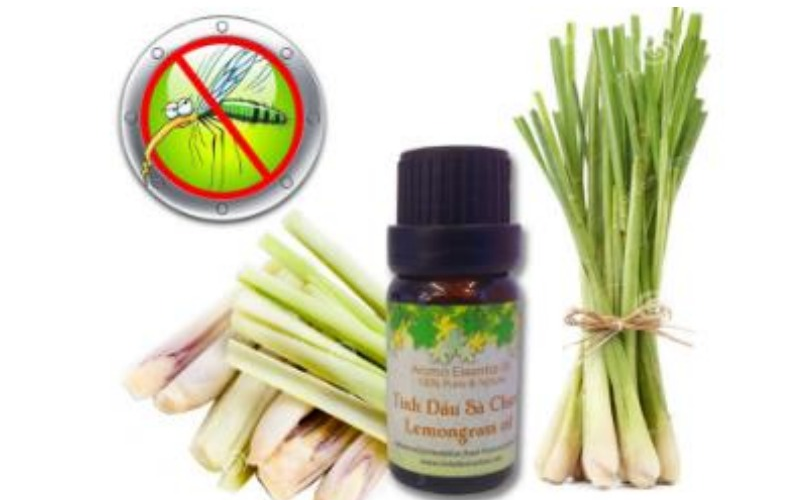
\includegraphics[width=6.5cm]{images_crop_hoa11_de09/cau12_p1_tinh_dau_sa.png}
\end{center}
\choice
{Chưng cất bằng hơi nước và chiết lại bằng nước lạnh}
{\True Chưng cất bằng hơi nước và chiết tinh dầu ra khỏi hỗn hợp sản phẩm}
{Chiết tinh dầu sả sau đó chưng cất bằng hơi nước}
{Kết tinh tinh dầu sả}

\loigiai{
Tinh dầu sả dễ bay hơi theo hơi nước và không tan trong nước, nhẹ hơn nước. Do đó dùng phương pháp chưng cất lôi cuốn hơi nước, sau đó ngưng tụ thu được hỗn hợp gồm nước và tinh dầu tách lớp, rồi dùng phễu chiết để tách tinh dầu ra khỏi nước.
}
\end{ex}

\begin{ex}
\textbf{[SBT - Cánh Diều]} Acetic acid có công thức phân tử là $\ce{C2H4O2}$. Kết luận nào sau đây là đúng?
\choice
{Acetic acid có công thức thực nghiệm là $\ce{CH2O}$ và có khối lượng riêng lớn hơn gấp 30 lần so với hydrogen ở cùng điều kiện}
{Acetic acid có công thức thực nghiệm là $\ce{CH2O}$ và có tỉ khối hơi so với hydrogen ở cùng điều kiện là 30}
{\True Acetic acid có công thức thực nghiệm là $\ce{CH2O}$ và có phân tử khối là 60}
{Acetic acid có công thức thực nghiệm là $\ce{(CH2O)2}$ và có phân tử khối là 60}

\loigiai{
$\ce{C2H4O2}$ có tỉ lệ số nguyên tử $\text{C} : \text{H} : \text{O} = 2 : 4 : 2 = 1 : 2 : 1$ nên công thức thực nghiệm (công thức đơn giản nhất) là $\ce{CH2O}$. Phân tử khối $M = 12 \times 2 + 4 \times 1 + 16 \times 2 = 60$.
}
\end{ex}

\begin{ex}
Trước kia, ``phẩm đỏ'' dùng để nhuộm áo choàng cho các Hồng y giáo chủ được tách chiết từ một loài ốc biển. Đó là một hợp chất có thành phần nguyên tố gồm: 45,7\% C; 1,90\% H; 7,60\% O; 6,70\% N và 38,10\% Br. Công thức phân tử (CTPT) của phẩm đỏ là: (Biết bằng phương pháp phổ khối lượng, người ta xác định được rằng trong phân tử ``phẩm đỏ'' có hai nguyên tử Br):
\choice
{\True $\ce{C16H8O2N2Br2}$}
{$\ce{C8H6ONBr}$}
{$\ce{C6H8ONBr}$}
{$\ce{C8H4ONBr2}$}

\loigiai{
Ta có tỉ lệ số mol các nguyên tố:
$$\text{C} : \text{H} : \text{O} : \text{N} : \text{Br} = \dfrac{45,7}{12} : \dfrac{1,9}{1} : \dfrac{7,6}{16} : \dfrac{6,7}{14} : \dfrac{38,1}{80} = 3,808 : 1,90 : 0,475 : 0,478 : 0,476 = 8 : 4 : 1 : 1 : 1.$$
Do đó công thức đơn giản nhất là $\ce{C8H4ONBr}$. Vì phân tử có 2 nguyên tử Br nên công thức phân tử là $(\ce{C8H4ONBr})_2 \Rightarrow \ce{C16H8O2N2Br2}$.
}
\end{ex}

\begin{ex}
Cho các chất sau: $\ce{CH3OH}$ (methanol), $\ce{CH3CH2OH}$ (a), $\ce{CH3CH2CH2OH}$ (b), $\ce{(CH3)2CHOH}$ (c), $\ce{(CH3)2CHCH2OH}$ (d), $\ce{(CH3)2CHCH2CH2OH}$ (e), $\ce{(CH3)3COH}$ (g), $\ce{HOCH2CH2OH}$ (h). Phát biểu nào sau đây là đúng?
\choice
{\True Các chất (a), (b), (c), (d), (e), (g) thuộc dãy đồng đẳng của methanol}
{Các chất (a), (b), (c), (d), (g), (h) thuộc dãy đồng đẳng của methanol}
{Các chất (a), (b), (d), (e), (g), (h) thuộc dãy đồng đẳng của methanol}
{Tất cả các chất đều thuộc dãy đồng đẳng của methanol}

\loigiai{
Methanol là alcohol no, đơn chức, mạch hở. Các chất (a), (b), (c), (d), (e), (g) đều là alcohol no, đơn chức, mạch hở có công thức chung $\ce{C_nH_{2n+1}OH}$ nên thuộc cùng dãy đồng đẳng của methanol. Chất (h) là alcohol hai chức (glycol) nên không cùng dãy đồng đẳng.
}
\end{ex}

\begin{ex}
\textbf{[SBT - KNTT]} Cho các phát biểu sau:
\begin{enumerate}[(1)]
	\item Công thức cấu tạo biểu diễn kiểu liên kết và trật tự liên kết giữa các nguyên tử trong phân tử;
	\item Chất đồng phân có cùng công thức phân tử nhưng có thể khác nhau về loại nhóm chức, mạch carbon, vị trí liên kết pi ($\pi$) hoặc vị trí nhóm chức;
	\item Chất đồng đẳng có cấu tạo và tính chất tương tự, nhưng thành phần phân tử khác nhau một hay nhiều nhóm $\ce{CH2}$.
\end{enumerate}
Số phát biểu đúng là
\choice
{0}
{1}
{2}
{\True 3}

\loigiai{
Cả 3 phát biểu (1), (2), (3) đều hoàn toàn chính xác theo định nghĩa về công thức cấu tạo, đồng phân và đồng đẳng.
}
\end{ex}

\begin{ex}
Ngâm rượu dược liệu: Cách tiến hành: Cho dược liệu vào trong lọ, bình hoặc hũ. Đổ một lượng rượu phù hợp rồi bịt kín lại đặt ở nơi tối, mát. Ngâm từ 10 -- 15 ngày, mùa đông có thể ngâm lâu hơn. Cho các phát biểu sau:
\begin{enumerate}[(1)]
	\item Ngâm dược liệu áp dụng phương pháp chiết lỏng -- rắn.
	\item Ngâm dược liệu áp dụng phương pháp chiết lỏng -- lỏng.
	\item Tách lấy chất hữu cơ ra khỏi một hỗn hợp ở thể rắn.
	\item Tách lấy chất hữu cơ ra khỏi một hỗn hợp ở thể lỏng.
\end{enumerate}
Số phát biểu đúng là
\choice
{\True 2}
{3}
{4}
{1}

\loigiai{
Ngâm rượu dược liệu là dùng dung môi ethanol hòa tan các hoạt chất hữu cơ có trong dược liệu thể rắn, đây là phương pháp chiết lỏng -- rắn (tách lấy chất hữu cơ ra khỏi hỗn hợp ở thể rắn). Vậy có 2 phát biểu đúng là (1) và (3).
}
\end{ex}

\begin{ex}
Cho các phát biểu:
\begin{enumerate}[(a)]
	\item Để tách ethanol và nước người ta sử dụng phương pháp chưng cất.
	\item Để tinh luyện đường đỏ thành đường trắng người ta sử dụng phương pháp kết tinh.
	\item Không thể tách tinh dầu chanh bằng phương pháp chưng cất và chiết.
	\item Phương pháp cột sắc kí thường dùng để tách các chất hữu cơ có hàm lượng nhỏ và khó tách.
	\item Phương pháp kết tinh được dùng để tách và tinh chế các chất rắn.
\end{enumerate}
Số phát biểu đúng là
\choice
{\True 4}
{3}
{2}
{1}

\loigiai{
Các phát biểu đúng gồm: (a), (b), (d), (e). Phát biểu (c) sai vì tinh dầu chanh hoàn toàn có thể tách được bằng phương pháp chưng cất lôi cuốn hơi nước kết hợp với chiết. Vậy có 4 phát biểu đúng.
}
\end{ex}

\Closesolutionfile{ans}
\newpage

\noindent\textbf{\large PHẦN II. Câu trắc nghiệm đúng sai.}
\textit{Thí sinh trả lời từ câu 1 đến câu 4. Trong mỗi ý a), b), c), d) ở mỗi câu, thí sinh chọn đúng hoặc sai.}
\vspace{0.2cm}

\begin{ex}
Trong bài báo khoa học ``Bioactive-Guided Phytochemical Investigations, In Vitro and In Silico Alpha-Glucosidase Inhibition of Two Vietnamese Medicinal Plants Dicranopteris linearis and Smilax glabra'', các nhà khoa học đã phân lập được hợp chất có công thức cấu tạo như sau từ loài dương xỉ \textit{Dicranopteris linearis}:
\begin{center}
	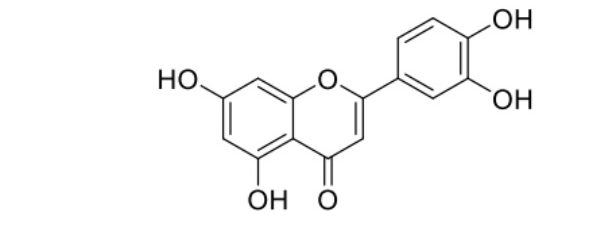
\includegraphics[width=6.5cm]{images_crop_hoa11_de09/cau1_p2_dicranopteris.png}
\end{center}
\choiceTF
{a) Hợp chất trên chứa nhóm chức alcohol}
{b) Hợp chất trên chứa nhóm chức carboxylic acid}
{\True c) Hợp chất trên chứa nhóm chức ketone}
{d) Hợp chất trên là hợp chất hữu cơ tổng hợp}

\loigiai{
\begin{itemize}
	\item a) \textbf{Sai}: Các nhóm $-\ce{OH}$ đều liên kết trực tiếp với vòng thơm benzene nên thuộc loại nhóm chức phenol, không phải alcohol.
	\item b) \textbf{Sai}: Trong cấu trúc không có nhóm chức carboxyl ($-\ce{COOH}$).
	\item c) \textbf{Đúng}: Nhóm $\ce{C=O}$ nằm trong vòng dị tố liên kết với hai nguyên tử carbon tạo thành nhóm chức ketone dạng cyclic enone.
	\item d) \textbf{Sai}: Hợp chất này được chiết xuất và phân lập từ thực vật tự nhiên (cây dương xỉ \textit{Dicranopteris linearis}), là hợp chất thiên nhiên.
\end{itemize}
}
\end{ex}

\begin{ex}
Nấu rượu thủ công là phương pháp truyền thống đã có từ lâu đời tại Việt Nam:
\begin{center}
	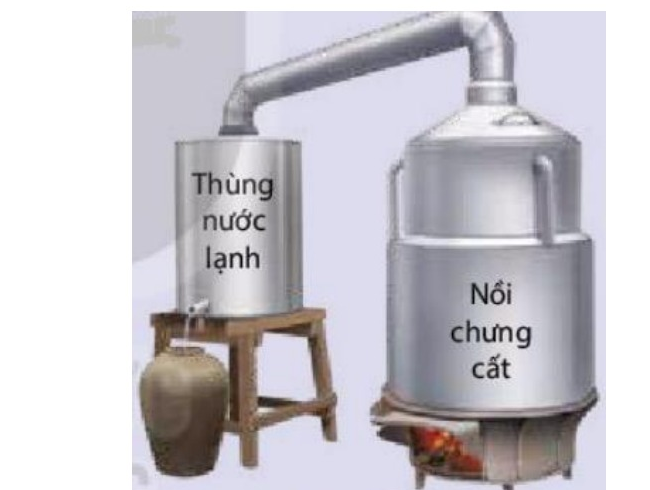
\includegraphics[width=7.5cm]{images_crop_hoa11_de09/cau2_p2_nau_ruou.png}
\end{center}
\choiceTF
{a) Rượu nấu xong chảy ra trước do nước có nhiệt độ sôi thấp hơn ethanol}
{\True b) Ống tre dẫn hơi rượu đi qua chậu nước lạnh nhằm mục đích ngưng tụ hơi ethanol thành thể lỏng}
{\True c) Phương pháp nấu rượu thủ công dựa trên sự khác nhau về nhiệt độ sôi của các chất trong hỗn hợp}
{d) Phương pháp tách chất trong quá trình nấu rượu thủ công thuộc phương pháp chưng cất phân đoạn}

\loigiai{
\begin{itemize}
	\item a) \textbf{Sai}: Ethanol có nhiệt độ sôi ($78,3^\circ\text{C}$) thấp hơn nước ($100^\circ\text{C}$) nên ethanol bay hơi trước và ngưng tụ chảy ra trước.
	\item b) \textbf{Đúng}: Hệ thống làm lạnh bằng nước giúp làm lạnh và ngưng tụ hơi ethanol cùng hơi nước thành chất lỏng (rượu).
	\item c) \textbf{Đúng}: Đây là nguyên lý của phương pháp chưng cất, tách các chất lỏng dựa vào độ bay hơi và nhiệt độ sôi khác nhau.
	\item d) \textbf{Sai}: Nấu rượu thủ công sử dụng thiết bị ngưng tụ đơn giản, thuộc phương pháp chưng cất thường (chưng cất đơn giản), không có tháp phân đoạn.
\end{itemize}
}
\end{ex}

\begin{ex}
Cho phổ khối lượng của hai hợp chất aniline ($\ce{C6H7N}$) và 2-aminopyridine ($\ce{C5H6N2}$) như sau:
\begin{center}
	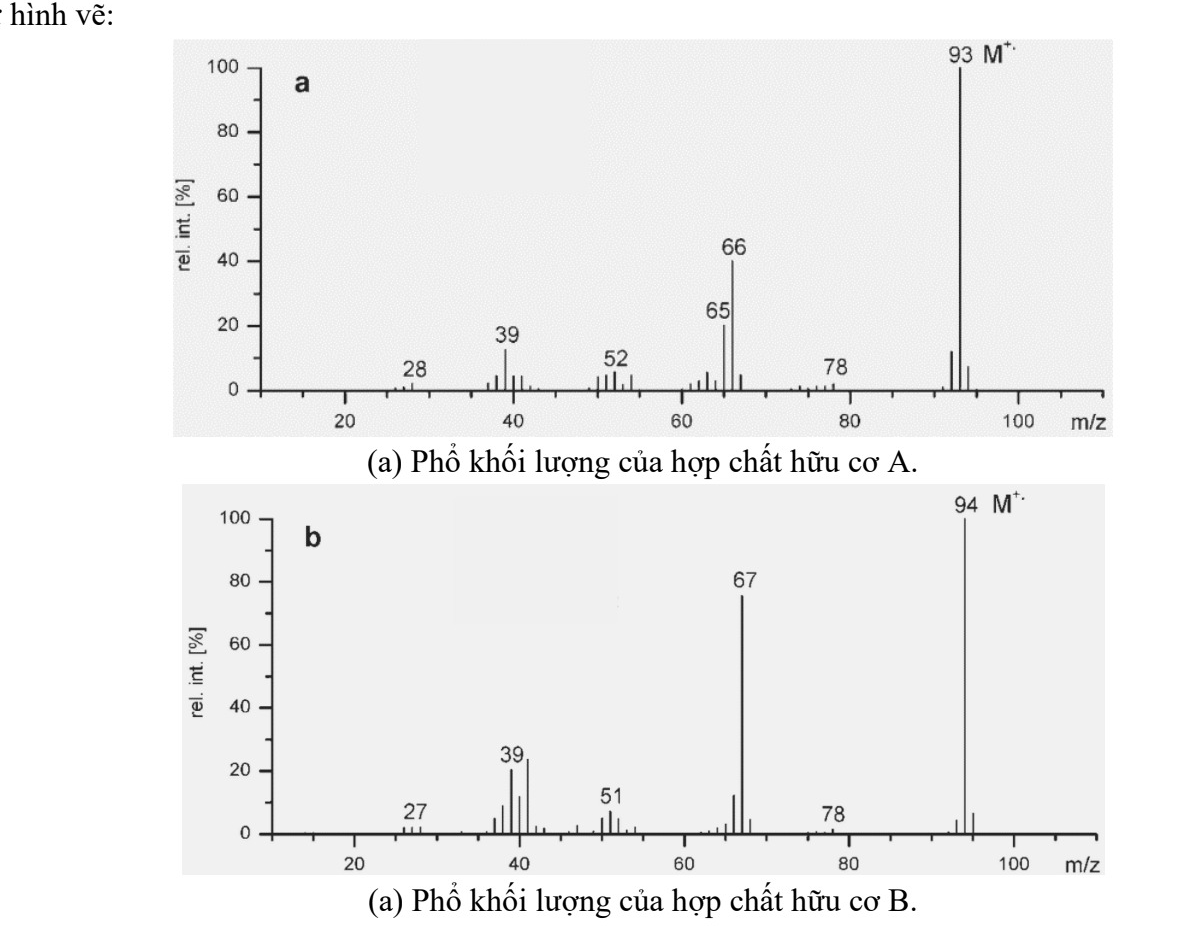
\includegraphics[width=11.0cm]{images_crop_hoa11_de09/cau3_p2_ms_aniline_aminopyridine.png}
\end{center}
\choiceTF
{\True a) Phổ khối lượng ở hình (a) tương ứng với phân tử aniline}
{b) Mảnh ion phân tử ở hình (b) có giá trị $m/z$ là 67}
{\True c) Phổ khối lượng ở hình (b) tương ứng với phân tử 2-aminopyridine}
{d) Phân tử khối của hai hợp chất hữu cơ A và B bằng nhau}

\loigiai{
\begin{itemize}
	\item a) \textbf{Đúng}: Aniline có công thức phân tử $\ce{C6H7N}$, phân tử khối $M = 12\times 6 + 7 + 14 = 93$. Trên phổ (a), pic ion phân tử $[\ce{M+}]$ có $m/z = 93$, tương ứng với aniline.
	\item b) \textbf{Sai}: Mảnh ion phân tử $[\ce{M+}]$ ở hình (b) có giá trị $m/z = 94$. Đỉnh tại $m/z = 67$ là mảnh ion phân đoạn (fragment ion) có cường độ tương đối cao nhất.
	\item c) \textbf{Đúng}: 2-Aminopyridine có công thức $\ce{C5H6N2}$, phân tử khối $M = 12\times 5 + 6 + 14\times 2 = 94$, ứng với đỉnh ion phân tử $[\ce{M+}]$ có $m/z = 94$ ở hình (b).
	\item d) \textbf{Sai}: Phân tử khối của aniline là 93 và của 2-aminopyridine là 94, hai giá trị phân tử khối này khác nhau.
\end{itemize}
}
\end{ex}

\begin{ex}
Citronellol là hợp chất được sử dụng tạo mùi hương tự nhiên có nguồn gốc từ các loại thực vật như hoa hồng, phong lữ hoặc sả, có công thức cấu tạo đầy đủ như sau:
\begin{center}
	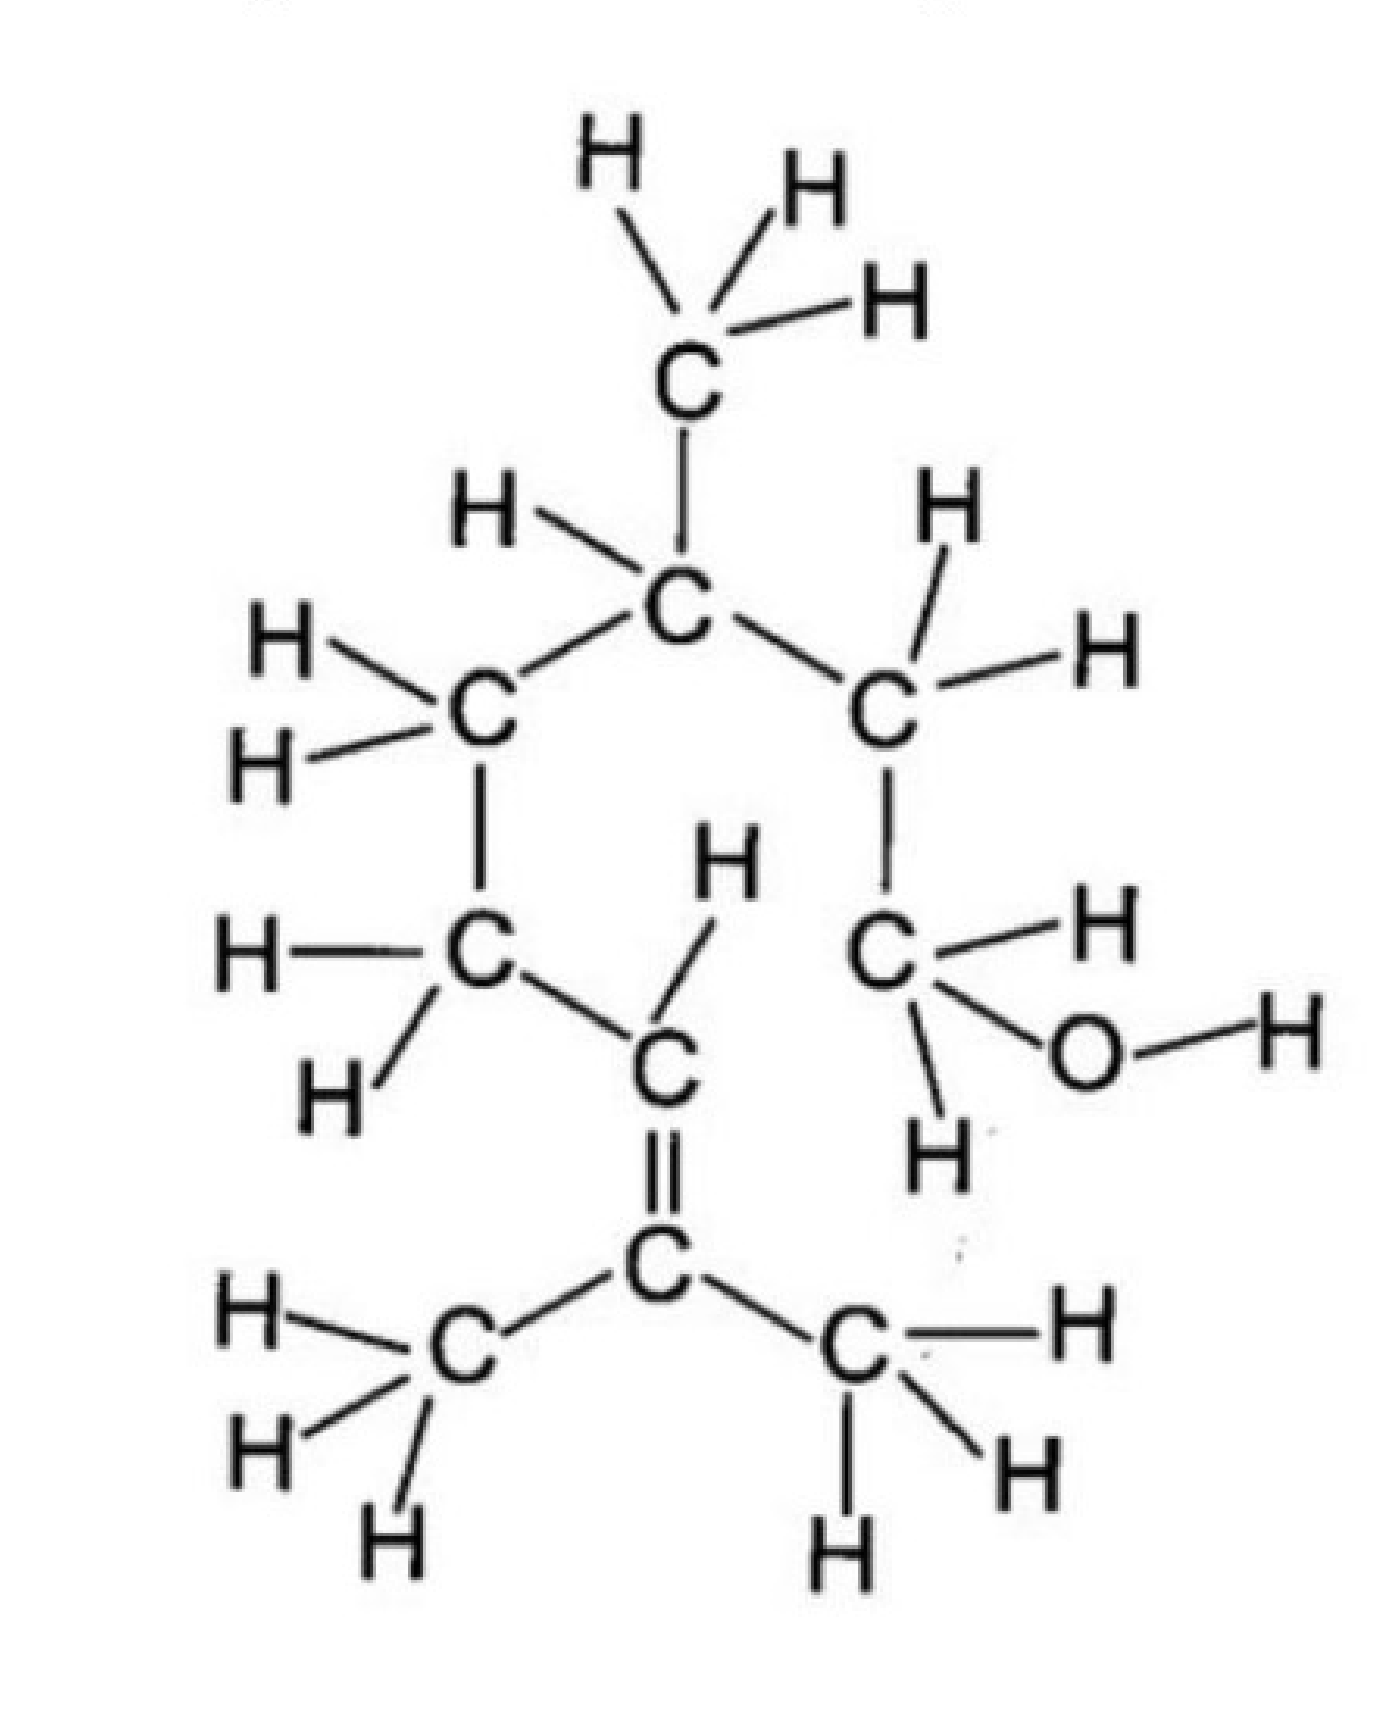
\includegraphics[width=4.5cm]{images_crop_hoa11_de09/cau4_p2_citronellol_full.png}
\end{center}
Cho 3 công thức cấu tạo sau:
\begin{center}
	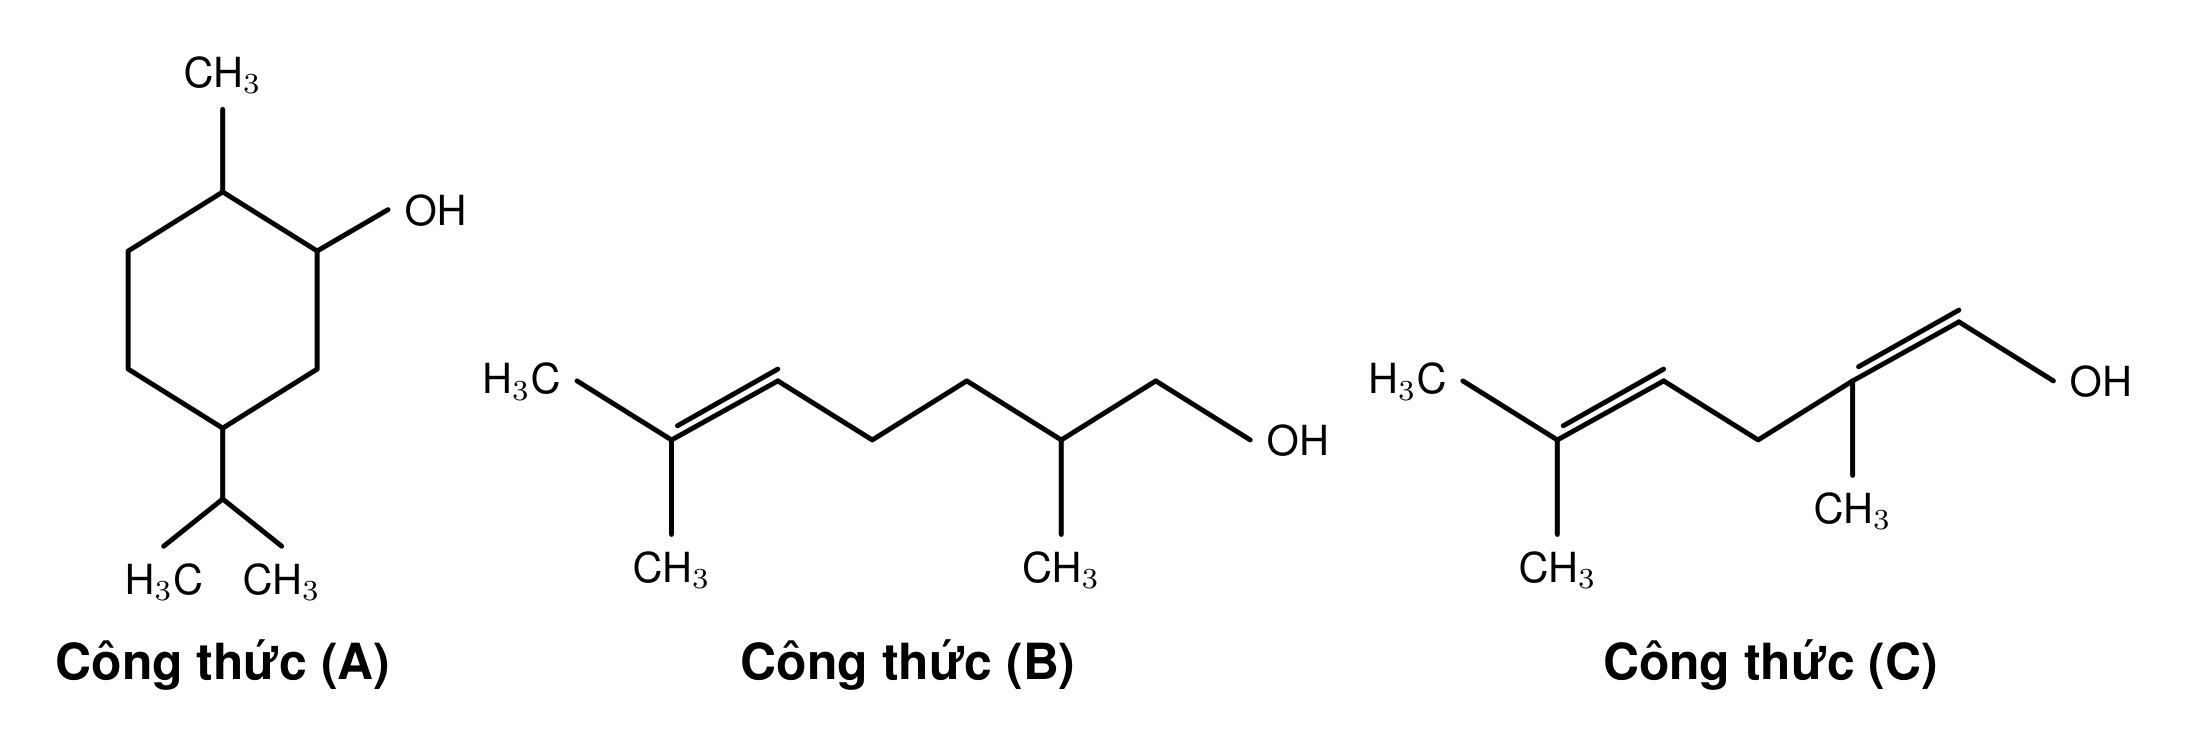
\includegraphics[width=13.5cm]{images_crop_hoa11_de09/cau4_p2_citronellol_ABC.png}
\end{center}
\choiceTF
{\True a) Trong các công thức (A), (B), (C) có đúng 1 công thức biểu diễn đúng citronellol}
{b) Citronellol có đồng phân hình học}
{\True c) Citronellol có khả năng phản ứng với Na giải phóng khí $\ce{H2}$}
{d) Citronellol thuộc loại hợp chất hữu cơ đa chức}

\loigiai{
\begin{itemize}
	\item a) \textbf{Đúng}: Chỉ có công thức (B) biểu diễn đúng cấu trúc mạch hở của citronellol: $\ce{(CH3)2C=CH-CH2-CH2-CH(CH3)-CH2-CH2-OH}$. Công thức (A) là menthol (vòng no 6 cạnh), công thức (C) là geraniol (chứa 2 liên kết đôi $\ce{C=C}$).
	\item b) \textbf{Sai}: Tại liên kết đôi $\ce{C=C}$, nguyên tử carbon số 7 liên kết với hai nhóm methyl ($-\ce{CH3}$) giống hệt nhau nên không thỏa mãn điều kiện có đồng phân hình học cis-trans.
	\item c) \textbf{Đúng}: Citronellol chứa nhóm chức alcohol bậc một ($-\ce{OH}$) có nguyên tử hydrogen linh động, tác dụng được với kim loại Na giải phóng $\ce{H2}$.
	\item d) \textbf{Sai}: Phân tử citronellol chỉ chứa duy nhất một nhóm chức alcohol ($-\ce{OH}$), do đó thuộc loại hợp chất đơn chức.
\end{itemize}
}
\end{ex}

\newpage
\noindent\textbf{\large PHẦN III. Câu trắc nghiệm yêu cầu trả lời ngắn.}
\textit{Thí sinh trả lời từ câu 1 đến câu 6.}
\vspace{0.2cm}

\begin{ex}
Cho các chất sau: $\ce{CH4}$, $\ce{C2H2}$, $\ce{CCl4}$, $\ce{C2H4}$, $\ce{C2H5OH}$, $\ce{CH3CHO}$. Có bao nhiêu chất là dẫn xuất của hydrocarbon?

\loigiai{
\textbf{Đáp số: 3}\\
Hydrocarbon chỉ chứa hai nguyên tố C và H: $\ce{CH4}$, $\ce{C2H2}$, $\ce{C2H4}$.\\
Dẫn xuất hydrocarbon ngoài C, H còn chứa các nguyên tố khác: $\ce{CCl4}$, $\ce{C2H5OH}$, $\ce{CH3CHO} \Rightarrow$ Có 3 chất.
}
\end{ex}

\begin{ex}
Cho các đặc điểm sau của sắc kí cột:
\begin{enumerate}[(1)]
	\item Pha tĩnh là chất rắn có diện tích bề mặt lớn, có khả năng hấp phụ khác nhau các chất trong hỗn hợp.
	\item Pha động là dung môi hữu cơ đi qua pha tĩnh mà không hòa tan các chất trong hỗn hợp.
	\item Các chất trong hỗn hợp được tách ra khỏi cột theo thứ tự khả năng bị hấp phụ tăng dần.
	\item Dung môi rửa giải chỉ được dùng một loại dung môi duy nhất trong suốt quá trình sắc kí.
	\item Sắc kí cột dùng để tách và tinh chế các chất hữu cơ có hàm lượng nhỏ hoặc khó tách bằng các phương pháp khác.
\end{enumerate}
Có bao nhiêu đặc điểm đúng?

\loigiai{
\textbf{Đáp số: 3}\\
Có 3 đặc điểm đúng là (1), (3), (5).\\
- Đặc điểm (2) sai vì pha động phải hòa tan và lôi cuốn các chất trong hỗn hợp di chuyển qua pha tĩnh.\\
- Đặc điểm (4) sai vì trong quá trình rửa giải có thể thay đổi dung môi hoặc tăng độ phân cực của dung môi để rửa giải các chất hấp phụ mạnh ra khỏi cột.
}
\end{ex}

\begin{ex}
Cho các chất sau: $\ce{C2H4O2}$, $\ce{C6H12O6}$, $\ce{C2H6O}$, $\ce{HCHO}$, $\ce{C3H6O2}$. Có bao nhiêu chất có cùng công thức đơn giản nhất là $\ce{CH2O}$?

\loigiai{
\textbf{Đáp số: 3}\\
Xét tỉ lệ $\text{C} : \text{H} : \text{O}$ của từng chất:\\
- $\ce{C2H4O2}$: $2 : 4 : 2 = 1 : 2 : 1 \Rightarrow \ce{CH2O}$ (thỏa mãn)\\
- $\ce{C6H12O6}$: $6 : 12 : 6 = 1 : 2 : 1 \Rightarrow \ce{CH2O}$ (thỏa mãn)\\
- $\ce{C2H6O}$: $2 : 6 : 1 \Rightarrow \ce{C2H6O}$\\
- $\ce{HCHO}$: $1 : 2 : 1 \Rightarrow \ce{CH2O}$ (thỏa mãn)\\
- $\ce{C3H6O2}$: $3 : 6 : 2 \Rightarrow \ce{C3H6O2}$\\
Vậy có 3 chất thỏa mãn.
}
\end{ex}

\begin{ex}
Trong cà rốt chứa hàm lượng cao $\beta$-caroten (tiền chất vitamin A), có công thức khung phân tử như sau:
\begin{center}
	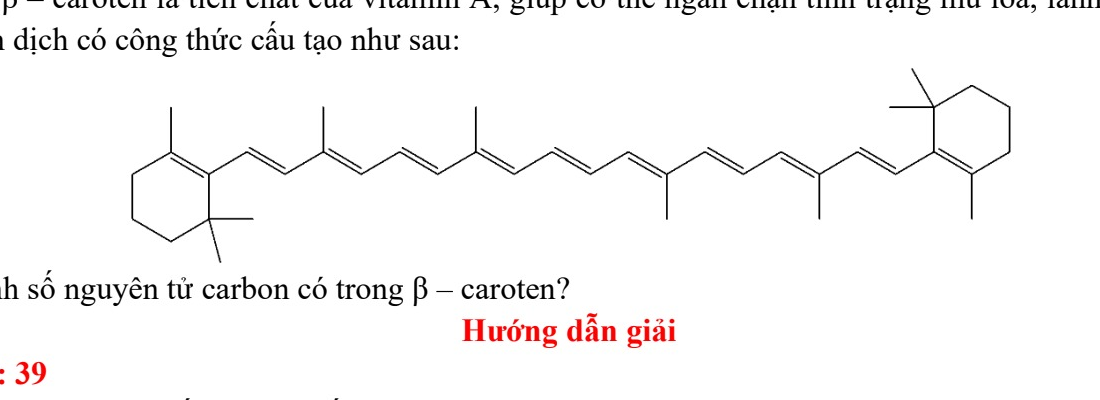
\includegraphics[width=11.5cm]{images_crop_hoa11_de09/cau4_p3_beta_caroten.png}
\end{center}
Số nguyên tử carbon trong một phân tử $\beta$-caroten là bao nhiêu?

\loigiai{
\textbf{Đáp số: 40 (hoặc 39 theo bản in gốc)}\\
$\beta$-Caroten là hợp chất tetraterpenoid đối xứng gồm 8 đơn vị isoprene (mỗi đơn vị 5C), công thức phân tử chuẩn là $\ce{C40H56}$, do đó số nguyên tử carbon chính xác trong phân tử là 40.\\
(\textit{Ghi chú: Trong đề in gốc có thể đếm thiếu 1 đỉnh carbon dẫn đến đáp số 39; đáp án chuẩn hóa học là 40}).
}
\end{ex}

\begin{ex}
Cây mía chứa khoảng 70\% nước ép, nước ép chứa khoảng 20\% saccharose ($\ce{C12H22O11}$). Từ 1 tấn mía, lượng saccharose kết tinh thu được là bao nhiêu kg (biết hiệu suất kết tinh đạt 80\%)?

\loigiai{
\textbf{Đáp số: 112}\\
Khối lượng nước ép mía thu được từ 1 tấn (1000 kg) mía là:
$$m_{\text{nước ép}} = 1000 \times 70\% = 700\text{ (kg)}.$$
Khối lượng saccharose có trong nước ép là:
$$m_{\text{saccharose}} = 700 \times 20\% = 140\text{ (kg)}.$$
Khối lượng saccharose kết tinh thực tế thu được ($H = 80\%$) là:
$$m_{\text{kết tinh}} = 140 \times 80\% = 112\text{ (kg)}.$$
}
\end{ex}

\begin{ex}
Acetone là dung môi hữu cơ quan trọng, thường dùng tẩy sơn móng tay. Phổ khối lượng của acetone cho thấy ion phân tử $[\ce{M+}]$ có $m/z = 58$ như hình vẽ:
\begin{center}
	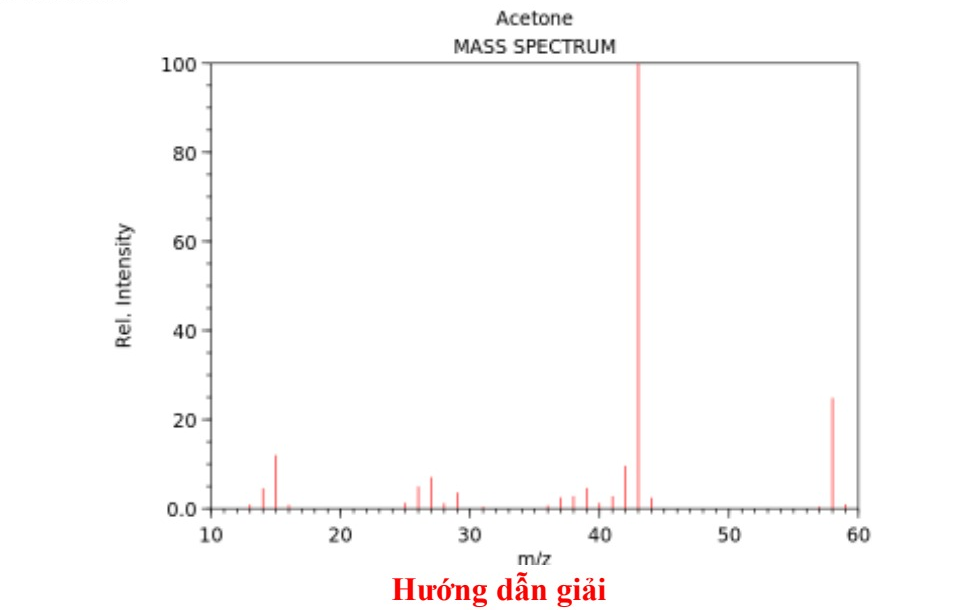
\includegraphics[width=7.5cm]{images_crop_hoa11_de09/cau6_p3_ms_acetone.png}
\end{center}
Biết công thức đơn giản nhất của acetone là $\ce{C3H6O}$. Tổng số nguyên tử trong một phân tử acetone là bao nhiêu?

\loigiai{
\textbf{Đáp số: 10}\\
Phổ khối lượng cho pic ion phân tử $[\ce{M+}]$ tại $m/z = 58 \Rightarrow$ Phân tử khối $M = 58$.\\
Công thức phân tử có dạng $(\ce{C3H6O})_n \Rightarrow (12\times 3 + 1\times 6 + 16)\times n = 58 \Rightarrow 58n = 58 \Rightarrow n = 1$.\\
Vậy CTPT của acetone là $\ce{C3H6O}$. Tổng số nguyên tử $= 3\ (\text{C}) + 6\ (\text{H}) + 1\ (\text{O}) = 10$.
}
\end{ex}

\vspace{0.2cm}
\noindent\textbf{\large PHẦN IV. Tự luận.}
\textit{Thí sinh trình bày lời giải chi tiết cho các câu hỏi sau.}
\vspace{0.2cm}

\begin{ex}
Cho các công thức khung cấu trúc sau đây:
\begin{center}
	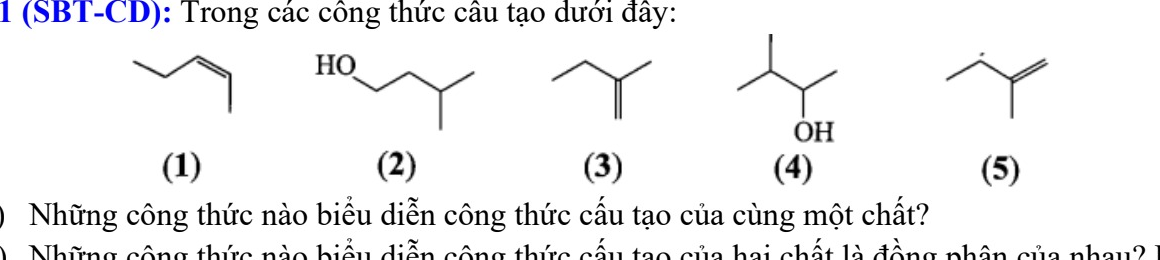
\includegraphics[width=11.5cm]{images_crop_hoa11_de09/cau1_p4_5khung_cau_truc.png}
\end{center}
\begin{enumerate}[a)]
	\item Hai công thức nào cùng biểu diễn một chất?
	\item Hai công thức nào là đồng phân cấu tạo vị trí nhóm chức của nhau?
\end{enumerate}

\loigiai{
\textbf{Hướng dẫn giải:}\\
\begin{itemize}
	\item a) Hai công thức cùng biểu diễn một chất:
	Công thức (3) và (5) cùng biểu diễn hydrocarbon có mạch chính 4 carbon, có 1 liên kết đôi ở đầu mạch và 1 nhóm methyl ở C2: 2-methylbut-1-ene ($\ce{CH2=C(CH3)-CH2-CH3}$).
	\item b) Hai công thức là đồng phân vị trí nhóm chức của nhau:
	Công thức (2) và (4) đều có cùng công thức phân tử $\ce{C5H12O}$ và cùng khung carbon 2-methylbutane, nhưng khác nhau về vị trí của nhóm chức alcohol ($-\ce{OH}$):
	\begin{itemize}
		\item Công thức (2): 3-methylbutan-2-ol (nhóm $-\ce{OH}$ ở carbon số 2).
		\item Công thức (4): 2-methylbutan-2-ol (nhóm $-\ce{OH}$ ở carbon số 2 đính kèm nhánh methyl).
	\end{itemize}
	Do đó, (2) và (4) là đồng phân vị trí nhóm chức của nhau.
\end{itemize}
}
\end{ex}

\begin{ex}
Một hợp chất hữu cơ X chứa 85,7\% C và 14,3\% H về khối lượng:
\begin{center}
	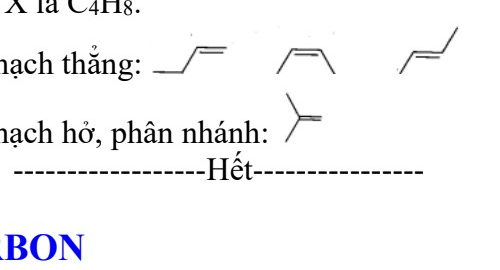
\includegraphics[width=6.5cm]{images_crop_hoa11_de09/cau2_p4_cau_truc_c4h8.png}
\end{center}
Phổ khối lượng cho thấy phân tử khối của X là 56.
\begin{enumerate}[a)]
	\item Xác định công thức thực nghiệm (công thức đơn giản nhất) của X.
	\item Xác định công thức phân tử của X.
	\item Viết công thức cấu tạo của X biết:
	\begin{itemize}
		\item[$c_1$.] X có mạch carbon không phân nhánh.
		\item[$c_2$.] X có mạch hở phân nhánh.
	\end{itemize}
\end{enumerate}

\loigiai{
\textbf{Hướng dẫn giải:}\\
\begin{enumerate}[a)]
	\item Đặt công thức đơn giản nhất của X là $\ce{C_xH_y}$.\\
	Ta có tỉ lệ số mol các nguyên tử:
	$$x : y = \dfrac{\%m_{\ce{C}}}{12} : \dfrac{\%m_{\ce{H}}}{1} = \dfrac{85,7}{12} : \dfrac{14,3}{1} = 7,14 : 14,3 = 1 : 2.$$
	Vậy công thức thực nghiệm (công thức đơn giản nhất) của X là $\ce{CH2}$.
	\item Công thức phân tử của X có dạng $(\ce{CH2})_n$.\\
	Theo phổ khối lượng, phân tử khối $M = 56 \Rightarrow 14n = 56 \Rightarrow n = 4$.\\
	Vậy công thức phân tử của X là $\ce{C4H8}$.
	\item Các công thức cấu tạo thỏa mãn:
	\begin{itemize}
		\item Trường hợp $c_1$: Mạch carbon không phân nhánh:
		\begin{itemize}
			\item Alkene mạch hở: $\ce{CH2=CH-CH2-CH3}$ (but-1-ene) hoặc $\ce{CH3-CH=CH-CH3}$ (but-2-ene, gồm đồng phân cis và trans).
			\item Cycloalkane vòng không phân nhánh: cyclobutane (vòng no 4 cạnh).
		\end{itemize}
		\item Trường hợp $c_2$: Mạch hở phân nhánh:
		\begin{itemize}
			\item 2-methylpropene (isobutylene): $\ce{CH2=C(CH3)2}$ hay $\ce{(CH3)2C=CH2}$.
		\end{itemize}
	\end{itemize}
\end{enumerate}
}
\end{ex}

\newpage
\begin{center}
	{\color{hfRed}\textbf{\Large BẢNG ĐÁP ÁN VÀ MA TRẬN ĐỀ SỐ 09}}
\end{center}

\smallskip
\noindent
\textbf{1. PHẦN I (Mỗi câu trả lời đúng thí sinh được 0,25 điểm):}
\begin{center}
\begin{tabular}{|c|c|c|c|c|c|c|c|c|}
\hline
\textbf{1. A} & \textbf{2. A} & \textbf{3. B} & \textbf{4. A} & \textbf{5. D} & \textbf{6. A} & \textbf{7. C} & \textbf{8. A} & \textbf{9. D} \\ \hline
\textbf{10. D} & \textbf{11. D} & \textbf{12. B} & \textbf{13. C} & \textbf{14. A} & \textbf{15. A} & \textbf{16. D} & \textbf{17. A} & \textbf{18. A} \\ \hline
\end{tabular}
\end{center}

\noindent
\textbf{2. PHẦN II (Trắc nghiệm đúng sai):}
\begin{itemize}
	\item \textbf{Câu 1:} a) Sai \quad|\quad b) Sai \quad|\quad c) Đúng \quad|\quad d) Sai
	\item \textbf{Câu 2:} a) Sai \quad|\quad b) Đúng \quad|\quad c) Đúng \quad|\quad d) Sai
	\item \textbf{Câu 3:} a) Đúng \quad|\quad b) Sai \quad|\quad c) Đúng \quad|\quad d) Sai
	\item \textbf{Câu 4:} a) Đúng \quad|\quad b) Sai \quad|\quad c) Đúng \quad|\quad d) Sai
\end{itemize}

\noindent
\textbf{3. PHẦN III (Trả lời ngắn):}
\begin{center}
\begin{tabular}{|c|c|c|c|c|c|}
\hline
\textbf{Câu 1} & \textbf{Câu 2} & \textbf{Câu 3} & \textbf{Câu 4} & \textbf{Câu 5} & \textbf{Câu 6} \\ \hline
3 & 3 & 3 & 40 (hoặc 39) & 112 & 10 \\ \hline
\end{tabular}
\end{center}

\begin{center}
\textbf{--------- HẾT ---------}
\end{center}

\end{document}
